\documentclass[a4paper,12pt, english]{article}
\usepackage[top=2cm, bottom=2cm, left=2cm, right=2cm]{geometry}
\usepackage{hyperref}
%\usepackage{babel}
\usepackage{amsmath}
\usepackage{setspace}

\usepackage{subcaption}

\usepackage{listings}
\usepackage{url}
\usepackage{graphicx}


\usepackage{caption}


\usepackage{enumitem}
\setlistdepth{9}
\setlist[enumerate,1]{label=\arabic*)}
\setlist[enumerate,2]{label=\Alph*)}
\setlist[enumerate,3]{label=\Roman*)}
\setlist[enumerate,4]{label=\arabic*)}
\setlist[enumerate,5]{label=\alph*)}
\setlist[enumerate,6]{label=\roman*)}
\setlist[enumerate,7]{label=\arabic*)}
\setlist[enumerate,8]{label=\alph*)}
\setlist[enumerate,9]{label=\roman*)}

\renewlist{enumerate}{enumerate}{9}

%\usepackage{enumitem}
%\setlistdepth{9}

%\onehalfspacing

%\makeatletter
%\ifnum \@itemdepth >5\@toodeep\else
%\makeatother



\begin{document}

\title{A List of Metrics from the expose2 Ontology (148 Classes)\\ \small{\url{http://expdb.cs.kuleuven.be/Expose.owl}}}
\date{10 Feb 2014}
\author{By: Noureddin Sadawi}
\maketitle

\large
\begin{enumerate}
\item \textbf{DM\_entity\_property}


\begin{enumerate}

\item \textbf{algorithm\_property}
	\begin{enumerate}
	\item \textbf{ qualitative\_algorithm\_property}
		\begin{enumerate}
		\item \underline{comprehensibility:} Is it easy for users to understand how the algorithm works and what it parameters do?
		\item \underline{cumulativity:} Algorithms which do not allow attributes to interact, such as naive Bayes have low cumulativity, while decision trees have high cumulativity, allowing maximal interaction between variables
		\item \textbf{ feature\_handling}
			\begin{enumerate}
			\item \underline{mixed\_feature\_handling}
			\item \underline{parallel\_feature\_handling}
			\item \underline{sequential\_feature\_handling}
			\end{enumerate}
		\item \underline{handles\_cost\_functions}
		\item \underline{handles\_nominal\_features}
		\item \underline{handles\_nominal\_target}
		\item \underline{handles\_numeric\_target}
		\item \underline{handles\_numerical\_features}
		\item \underline{handles\_relational\_data}
		\item \underline{incrementality:} An algorithm is incremental if it can build and refine a model gradually as new training instances come in, without reexamining all instances seen in the past. However, they are generally very sensitive to the order in which examples are presented.
		\item \underline{interpretability:} Whether the model can be interpreted to extract knowledge. For instance, a decision tree is easy to interpret by humans, a neural network is not.
		\item \textbf{ model\_refinement\_procedure}
			\begin{enumerate}
			\item \underline{hypothesis\_optimization:} An hypothesis optimization learner is an inductive algorithm that assumes the data can be correctly modelled by a given mathematical function, and that adjusts that function (e.g. by adjusting weights) to fit the given data optimally. Examples are linear regression, backpropagation in artificial neural networks, Bayes rule in Bayesian methods and the kernel trick in kernel methods. 
			\item hypothesis\_refinement: An hypothesis refinement learner is an inductive algorithm that assumes the data can be correctly modelled by a given model, and that incrementally adjusts that model as it sees new data points (observations). Examples are decision tree learners, covering learners (rule learners), kMeans and logical induction. 
			\end{enumerate}
		\item \underline{optimizability:} The degree to which model and search parameters are handled automatically, or how much work goes into fine-tuning all parameter settings. Naive Bayes is very simple to tune, Support Vector Machines are much harder to optimize
		\item \underline{performs\_classification}
		\item \underline{performs\_regression}
		\item \underline{representational\_model}
		\end{enumerate}
	\item \textbf{ quantitative\_algorithm\_property}
		\begin{enumerate}
		\item \underline{bias-variance\_profile:} Bias and variance can be measured only with regard to the expectation of a learned models actual output, averaged over the ensemble of possible training sets D for a fixed sample size N. We thus need to evaluate algorithms on many different equally-sized samples of the same dataset, and repeat this process over many datasets in order to assess the average percentage of bias error versus variance error typically observed in the algorithm. If an algorithm has parameters that influence its bias, then we must take these into account as well.
		\item \underline{resilience\_to\_irrelevant\_attributes}
		\item \underline{resilience\_to\_missing\_values}
		\item \underline{resilience\_to\_noise}
		\item \underline{resilience\_to\_redundant\_attributes}
		\item \underline{scalability:} A learning algorithm is scalable if it performs as well on large datasets as it does on smaller ones. A systematic profiling should include the dimensions of the dataset, such as the number of examples, the number of attributes, and in case of classification, the number of classes. 
		\item \underline{space\_complexity}
		\item \underline{time\_complexity}
		\end{enumerate}
	\end{enumerate}
\item \textbf{data\_property}
\begin{enumerate}
	\item \textbf{ dataset\_property}
		\begin{enumerate}
		\item \textbf{ qualitative\_dataset\_property}
			\begin{enumerate}
			\item \textbf{ data\_cleanliness}
				\begin{enumerate}
				\item \underline{contains\_missing\_values}
				\item \underline{missing\_value\_free}
				\end{enumerate}
			\item \textbf{supervision}
				\begin{enumerate}
				\item \underline{semi-supervised}
				\item \underline{supervised}
				\item \underline{unsupervised}
				\end{enumerate}
			\end{enumerate}
		\item \textbf{quantitative\_dataset\_property}
			\begin{enumerate}
			\item \textbf{concept-based\_dataset\_property}
				\begin{enumerate}
				\item \underline{concept\_variation:} the (non-) uniformity of the class-label distribution throughout the feature space (measured through the distance between two examples of a different class)
				\item \underline{example\_cohesiveness:}  the density of the example distribution in the training set
				\end{enumerate}			
			\item \textbf{information\_theoretic\_dataset\_property}
				\begin{enumerate}
				\item \underline{average\_mutual\_information}
				\item \underline{coefficient\_of\_variation\_of\_target:} The coefficient of variation of the target is defined as the ratio of the standard deviation to the mean of the target attribute and can be used instead of entropy on numerical targets. It is a normalization of the standard deviation of the target useful for numerical targets $X_{target}$. A related measure, \emph{sparsity of the target}, is $VarCoef_{target}$ discretized into 3 values. \begin{equation} VarCoef_{target}=\frac{\sigma_{X}}{\mu_{X}} \end{equation}
				\item \underline{equivalent\_number\_of\_attributes:} The equivalent number of attributes is a quick estimate of the number of attributes required, on average, to describe the class. \begin{equation} EN-atrr=\frac{H(C)}{\overline{MI(C,X)}} \end{equation}
				\item \underline{median\_of\_uncertainty\_coefficients}
				\item \underline{noise\_to\_signal\_ratio:} The noise to signal ratio is an estimate of the amount of non-useful information in the attributes regarding the class. $\overline{H(X)}$ is the average information (useful or not) of the attributes. \begin{equation} NS-ratio=\frac{\overline{H(X)}-\overline{MI(C,X)}}{\overline{MI(C,X)}} \end{equation}
				\item \underline{target\_feature\_entropy}
				\end{enumerate}			
			\item \textbf{instance-based\_property:} Compares entire instances with each other. A dataset may contain two observations with similar or equal attribute values, but with different labels which might cause a classifier to get ‘confused’. Analogously, there might be two or more observations which are identical, which (unfairly?) gives them more weight in some algorithms. Here, properties derived from case-based learning are used originally intended to assess the quality of a given case-base.
				\begin{enumerate}
				\item \underline{instance\_consistency:} A single example is consistent within the dataset if and only if there does not exist any other example that is identical, but has a different target value
				\item \underline{instance\_incoherence:} Incoherence is a measure for how dissimilar the examples are in their attribute space. An example is called incoherent within a dataset if it does not overlap with any other example in a predefined number δ of attributes.
				\item \underline{instance\_minimality:} An example is subsumed by another example if its attributes form a true subset of another example with the same label. It is useful mostly for relational representations. An example that is not subsumed by another example is minimal. 
				\item \underline{instance\_similarity:}  The overall similarity of examples in a dataset is defined as the normalized weighted sum of four different local similarity measures
				\item \underline{instance\_uniqueness:} An example is unique if and only if there does not exist another identical example.
				\end{enumerate}			
			\item \textbf{landmarker:} A different way of probing the structure of the concepts hidden in the data is running some algorithms on it with very different biases, and see how well they perform: the better they do, the closer their bias fits the data. This is what is done naturally when we manually seek an appropriate algorithm: we first select a wide range of very different algorithms, do some preliminary evaluations, and then we remove all algorithms that don’t seem to perform well, leaving us with a small set of candidates to evaluate in detail.
				\begin{enumerate}
				\item \underline{1-nearest\_neighbor\_landmarker:}  Define a distance on the instance space, e.g. the euclidean distance, and label new observation with the observation of the closest training example. In classification problems, the goal of this landmark learner is to determine how close instances belonging to the same class are.
				\item \underline{decision\_stump\_landmarker:} Using a decision tree learner, C5.0 to be precise, a single decision node is constructed (representing a single split of the data) which is then to be used for classifying test observations. The goal of this landmark learner is to establish closeness to linear separability.
				\item \underline{elite\_1-nearest\_neighbor\_landmarker:}  A 1-Nearest Neighbor is used again, but only on a subset of attributes, i.e. the most informative attributes according to the information gain ratio. It intents to establish whether a task involves parity-like relationships between its attributes, which means that no single attribute is considerably more informative than another.
				\item \underline{linear\_discriminant\_landmarker:}  A single linear target function is computed splitting the instance space in two. Like decision stumps, it also establish closeness to linear separability, but not axis-parallel as is the case in the former.
				\item \underline{naive\_Bayes\_landmarker:}  A simple learning algorithm using Bayes’ theorem to calculate the possibility that an observation belongs to a certain class. Since it assumes that the attributes are conditionally independent from each other, this landmarker is used to measure the extent to which the attributes actually are independent given the class.
				\item \underline{random\_tree\_landmarker:}  Also using decision trees, an attribute is chosen randomly at each node until the entire tree is built. The goal of this landmark learner is to inform about irrelevant attributes.
				\item \underline{worst\_node\_landmarker:} By using the decision tree’s information gain ratio again, the least informative attribute is used to make the single split. Together with the first landmark learner, this landmarker is supposed to inform about linear separability.
				\end{enumerate}			
			\item \textbf{model-based\_property:} model-based characterization, builds a model that is typically very fast to induce, and characterizes the data based on properties of that model without doing a full-fletched evaluation of a wide range of learning algorithms.
				\begin{enumerate}
				\item \textbf{decision\_tree-based\_property:}
					\begin{enumerate}
					\item \underline{distribution\_of\_branch\_lengths}
					\item \underline{distribution\_of\_feature\_occurrence\_in\_nodes\_}
					\item \underline{distribution\_of\_number\_of\_nodes\_per\_level}
					\item \underline{number\_of\_leafs}
					\item \underline{number\_of\_nodes}
					\item \underline{tree\_depth}
					\item \underline{tree\_width}
					\end{enumerate}				
				\end{enumerate}			
			\item \textbf{simple\_dataset\_property:}
				\begin{enumerate}
				\item \underline{dimensionality\_of\_the\_data:} ratio of number\_of\_attributes and number\_of\_instances
				\item \underline{number\_of\_binary\_features}
				\item \underline{number\_of\_features}
				\item \underline{number\_of\_instances}
				\item \underline{number\_of\_instances\_with\_missing\_values}
				\item \underline{number\_of\_missing\_values}
				\item \underline{number\_of\_nominal\_features}
				\item \underline{number\_of\_numerical\_features}
				\item \underline{number\_of\_target\_classes}
				\item \underline{percentage\_of\_features\_with\_outliers}
				\item \underline{percentage\_of\_missing\_values}
				\item \underline{percentage\_of\_nominal\_features}
				\item \underline{percentage\_of\_numerical\_features}
				\item \underline{presence\_of\_outliers\_in\_target}
				\end{enumerate}			
			\item \textbf{statistical\_dataset\_property}
				\begin{enumerate}
				\item \underline{average\_correlation\_to\_target:} Measures the correlation between a numerical attribute $X$ and a numerical target $Y_{target}$.
				\item \underline{average\_feature\_kurtosis}
				\item \underline{average\_feature\_skewness}
				\item \underline{average\_p-value\_for\_target:} measures the correlation between a nominal attribute $X$ and a numerical target $Y_{target}$.
				\item \underline{Box's\_M\_statistic:} Box's M-statistic measures the equality of the covariance matrices $S_{i}$ of the different classes. If they are equal, then linear discriminants could be used, otherwise, quadratic discriminant functions should be used instead. As such, $M$ predicts whether a linear discriminant algorithm should be used or not. In the following, $S_{i}=\frac{S_{c_{i}}}{n_{i}-1}$ is the $i$ class covariance matrix with $S_{c_{i}}$ the $i$ class scatter matrix and $n_{i}$ the number of examples pertaining to class $i$, and $S=\frac{1}{n-cl}\sum_{i}S_{c_{i}}$ the pooled covariance matrix. It is zero when all individual covariance matrices are equal to the pooled covariance matrix. \begin{eqnarray} M&=&\gamma\sum_{i}(n_{i}-1)log\frac{|S|}{|S_{i}|} \\ \gamma&=&1-\frac{2num^{2}+3num-1}{6(num+1)(cl-1)}(\sum_{i}\frac{1}{n_{i}-1}-\frac{1}{n-cl}) \end{eqnarray}
				\item \underline{first\_canonical\_correlation:}  the first canonical correlation coefficient measures the association between all numerical attributes and a nominal (class) attribute. In principal component analysis (PCA), datasets are transformed into a new dataset with fewer dimensions (attributes). The first dimension, called the first principal component is a new axis in the direction of maximum variance. The variance of this principal axis is given by the largest eigenvalue $\lambda_{1}$. It thus measures how well the classes can be separated by the numerical attributes. \begin{equation} \rho_{max}=\sqrt{\frac{\lambda_{1}}{1+\lambda_{1}}} \end{equation}
				\item \underline{frac1:} the fraction of the total variance retained in the 1-dimensional space defined by the first principal component can be computed as the ratio between the largest eigenvalue $\lambda_{1}$ of the covariance matrix S and the sum of all its eigenvalues: \begin{equation} frac1=\frac{\lambda_{1}}{\sum_{i}\lambda_{i}} \end{equation}
				\item \underline{SD-ratio:} SD-ratio, the standard deviation ratio, is a reexpression of Box's M-statistic $M$ which is one if $M$ is zero and strictly greater than one if the covariances differ. \begin{equation} SD\mbox{-}ratio=exp(\frac{M}{num\sum_{i}(n_{i}-1)}) \end{equation}
				\item \underline{stationarity\_of\_target:} Indicates whether the standard deviation of the target feature is larger that its mean 
				\item \underline{target\_feature\_kurtosis}
				\item \underline{target\_feature\_skewness}
				\end{enumerate}			
			\item \textbf{sub-sampling\_landmarker:} Runs the learning algorithms on a small sample of the data, which for most algorithms will result in much faster training times. Indeed, learning algorithms typically learn the most from the first few examples. More examples will further fine-tune the model, but the performance gains will be small in comparison with the first few examples. When plotting the performance of learning algorithms on increasingly larger samples of a dataset, the resulting curve is called a learning curve. It will typically shoot up after a small percentage of the data and will, depending on the learning algorithm, start to level off shortly after that. The assumption of subsampling landmarking is that the performance of one point in the beginning of the learning curve will help us to predict the performance on the entire dataset.
				\begin{enumerate}
				\item \underline{partial\_learning\_curve}
				\item \underline{single\_subsample}
				\end{enumerate}			
			\item \textbf{task-specific\_dataset\_property:}
				\begin{enumerate}
				\item \underline{clustering\_dataset\_property}
				\item \textbf{time\_series\_analysis\_dataset\_property:}
					\begin{enumerate}
					\item \underline{coefficient\_of\_variation}
					\item \underline{mean\_of\_first\_5\_autocorrelations}
					\item \underline{statistical\_significance\_of\_autocorrelations}
					\end{enumerate}				
				\end{enumerate}			
			\end{enumerate}
		\end{enumerate}
	\item \textbf{feature\_property:}
		\begin{enumerate}
		\item \textbf{qualitative\_feature\_property:}
			\begin{enumerate}
			\item \textbf{feature\_datatype:}
				\begin{enumerate}
				\item \underline{nominal\_datatype}
				\item \textbf{numerical\_datatype:}
					\begin{enumerate}
					\item \underline{boolean\_datatype}
					\item \underline{integer\_datatype}
					\item \textbf{real\_datatype:}
						\begin{enumerate}
						\item \underline{real\_from\_0\_to\_1\_datatype}
						\end{enumerate}					
					\end{enumerate}				
				\end{enumerate}			
			\end{enumerate}		
		\item \textbf{quantitative\_feature\_property:}
			\begin{enumerate}
			\item \underline{feature\_entropy:} the entropy of a nominal attribute X is a measure of the uncertainty (or randomness) associated with it. It measures the average information content one is missing when one does not know the exact value of X. If entropy is zero (if all values are the same), the attribute contains no information. The class entropy H(C) is the amount of information required to specify the class of an instance, a measure for how ‘informative’ the attributes need to be. A low H(C) means that the distribution of examples among classes is very skewed (containing some very infrequent classes) which some algorithms cannot handle well. \begin{equation} H(X)_{norm}=\frac{H(X)}{log_{2}n} \end{equation} Although a definition exists for numerical distributions (using an integral instead of a summation), it is of no use for empirical data, and the entropy of numerical attributes (or targets) is calculated by discretizing the values in equal-length intervals.
			\item \underline{feature\_kurtosis:}  $\beta$, the kurtosis or fatness of the distribution's tail, or the 4th standardized moment \begin{equation} \beta=\frac{E(X-\mu_{X})^{4}}{\sigma_{X}^{4}} \end{equation}
			\item \textbf{feature\_redundancy\_property:} Determines the degree of redundancy in a dataset: if two or more attributes are dependent, they don't add much information and only increase the dimensionality of the dataset. This is measured by estimating the strength of the relationship between attributes.
				\begin{enumerate}
				\item \underline{feature\_concentration\_coefficient:} $\tau_{XY}$, the \emph{concentration coefficient} measuring the association between two nominal attributes, or the proportional reduction in the probability of an incorrect guess predicting $Y$, with $J$ distinct values, using $X$, with $I$ distinct values \begin{equation} \tau_{XY}=\frac{\sum_{i}\sum_{j}\frac{\pi^{2}_{ij}}{\pi_{i+}}-\sum_{j}\pi^{2}_{+j}}{1-\sum_{j}\pi^{2}_{+j}} \end{equation}
				\item \underline{feature\_correlation\_coefficient:} $\rho_{XY}$, the correlation coefficient measuring the association between two numerical attributes \begin{equation} \rho=\frac{\sigma_{XY}}{\sqrt{\sigma_{X}^{2}\sigma_{Y}^{2}}} \label{eq:rho} \end{equation}
				\item \underline{multiple\_correlation\_coefficient:} $R_{i}$, the multiple correlation coefficient measuring the maximal correlation coefficient between a numerical attribute $X_{i}$ and some linear combination of all other numerical attributes $Z_{i}\alpha$, with $Z_{i}=(X_{1},\ldots,X_{i-1},$ $X_{i+1},$ $\ldots,X_{num})$ and $\alpha$ a non-zero vector. \begin{equation} R_{i}=argmax_{\alpha\neq0} \frac{\sigma_{X_{i}Z_{i}\alpha}} {\sqrt{\sigma_{X_{i}}^{2}\sigma_{Z_{i}\alpha}^{2} } } \end{equation}
				\item \underline{mutual\_information:} $MI(Y,X)$, the \emph{mutual information} between nominal attributes $X$ and $Y$ describes the reduction in uncertainty of $Y$ due to the knowledge of $X$, and leans on the conditional entropy $H(Y|X)$. It is also the underlying measure of the information gain metric used in decision tree learners. \begin{eqnarray} MI(Y,X)&=&H(Y)-H(Y|X) \\ H(Y|X)&=&\sum_{i}p(X=x_{i})H(Y|X=x_{i}) \\ &=&-\sum_{i}\pi_{i+} \sum_{j}\pi_{j|i}log_{2}(\pi_{j|i}) \end{eqnarray}
				\item \underline{p-value\_of\_F\_distribution:} $p_{val_{XY}}$, the p-value of the F-distribution for a nominal attribute $X$ with $I$ values and a numeric attribute $Y$. The Analysis of Variance (ANOVA) examines how a numerical variable affects a nominal one by examining whether the means of the $I$ groups defined on $Y$ by $X$ are different. The ratio of the \emph{between group variance} and the \emph{within group variance} $MS(B)/MS(W)$ follows the F-distribution and the p-value of that distribution gives the probability of observing that ratio under the assumption that the group means are equal. A p-value close to one means we can accept that assumption, an indication that $X$ heavily affects $Y$
				\item \underline{uncertainty\_coefficient:} $UC(X,Y)$, the uncertainty coefficient is the mutual information between an attribute $X$ and target attribute $Y$ divided by the entropy of $Y$. It measures the proportional reduction in the \emph{variance} of $Y$ when $X$ is known. It is strongly related to the \emph{information gain ratio} used in decision trees, which is defined as $UC(Y,X)$, or the proportional reduction in in the variance of $X$ when target $Y$ is known. \begin{equation} UC(X,Y)=\frac{MI(Y,X)}{H(X)} \end{equation}
				\end{enumerate}			
			\item \underline{feature\_skewness:} $\gamma$, the skewness or lack of symmetry in the distribution, or the 3rd standardized moment \begin{equation} \gamma=\frac{E(X-\mu_{X})^{3}}{\sigma_{X}^{3}} \end{equation}
			\item \textbf{nominal\_feature\_properties:}
				\begin{enumerate}
				\item \underline{number\_of\_feature\_values}
				\end{enumerate}			
			\item \underline{normalized\_feature\_entropy:}  $H(X)_{norm}$, the normalized entropy of a nominal attribute $X$ rescales entropy to the [0..1] interval \begin{equation} H(X)_{norm}=\frac{H(X)}{log_{2}n} \end{equation} 
			\item \textbf{numerical\_feature\_properties:}
				\begin{enumerate}
				\item \underline{maximum\_feature\_value}
				\item \underline{minimum\_feature\_value}
				\end{enumerate}			
			\end{enumerate}		
		\end{enumerate}
	\item \textbf{instance\_property:}
		\begin{enumerate}
		\item \textbf{labeling:}
			\begin{enumerate}
			\item \underline{labeled}
			\item \underline{unlabeled}
			\end{enumerate}		
		\end{enumerate}	
\end{enumerate}

\end{enumerate}

\item \textbf{machine\_property:}
	\begin{enumerate}
	\item \underline{amount\_of\_memory}
	\item \underline{benchmark\_speed}
	\item \underline{cpu\_speed}
	\item \underline{number\_cpus}
	\end{enumerate}
\end{enumerate}
\newpage

\begin{figure}[h]   
  \centering 
  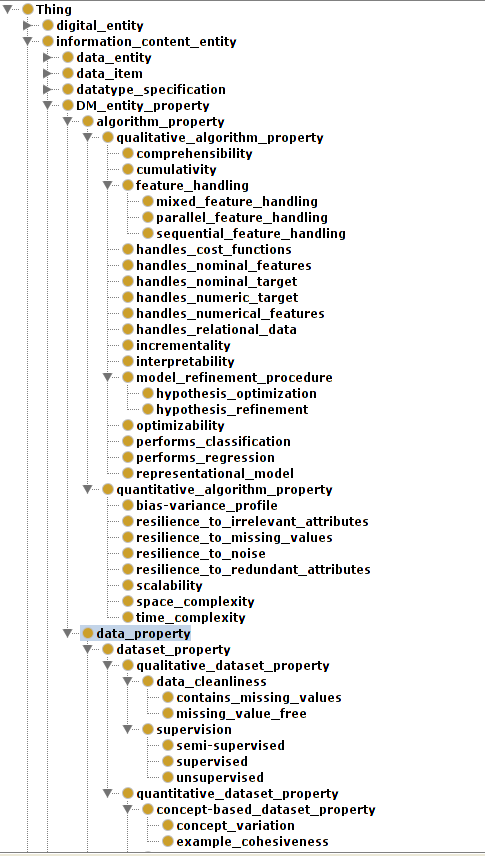
\includegraphics[width=0.75\textwidth]{../figs/expose2-1}
  \caption{}
  \label{fig:expose2-1}
\end{figure}

\begin{figure}[h]   
  \centering 
  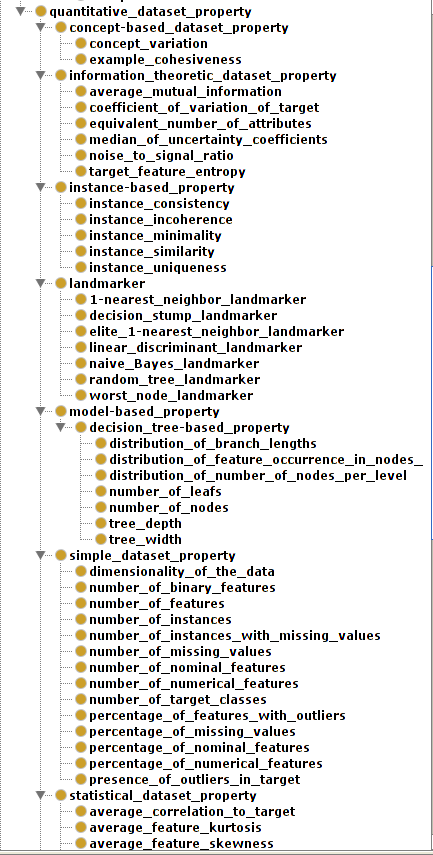
\includegraphics[width=0.75\textwidth]{../figs/expose2-2}
  \caption{}
  \label{fig:expose2-2}
\end{figure}

\begin{figure}[h]   
  \centering 
  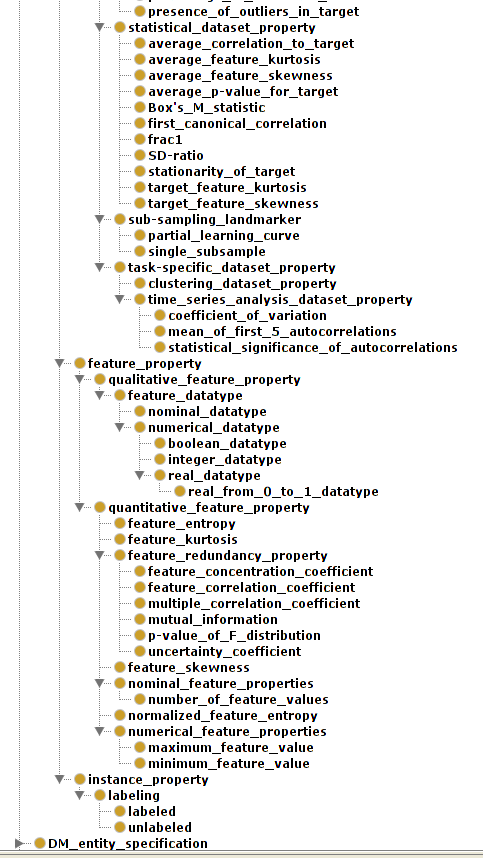
\includegraphics[width=0.75\textwidth]{../figs/expose2-3}
  \caption{}
  \label{fig:expose2-3}
\end{figure}

\begin{figure}[h]   
  \centering 
  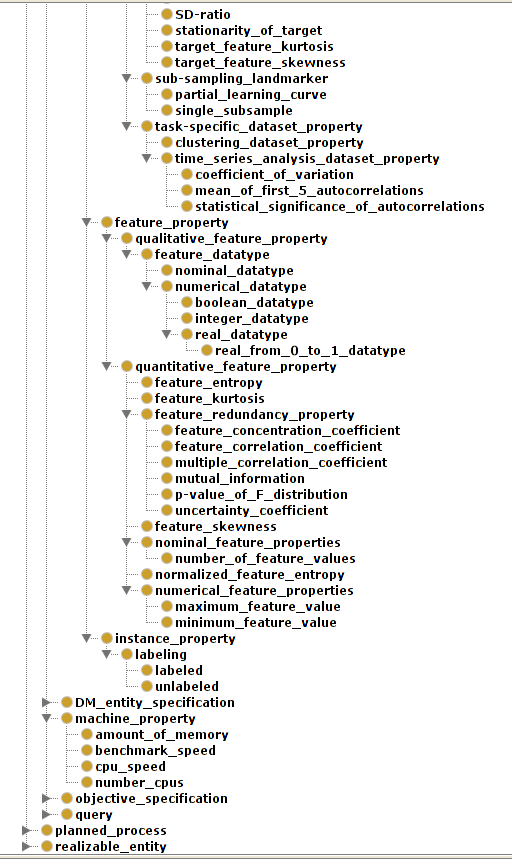
\includegraphics[width=0.875\textwidth]{../figs/expose2-4}
  \caption{}
  \label{fig:expose2-4}
\end{figure}


\end{document}
